\documentclass{article}
\usepackage{arxiv}
\usepackage[utf8]{inputenc}
\usepackage[english, russian]{babel}
\usepackage[T1]{fontenc}
\usepackage{url}
\usepackage{booktabs}
\usepackage{amsfonts}
\usepackage{nicefrac}
\usepackage{microtype}
\usepackage{lipsum}
\usepackage{graphicx}
\usepackage{natbib}
\usepackage{doi}



\title{Polarization detection of texts in the news flow}

\author{Роман Авдеев \\
	Студент 4 курса 417 гр.\\
	Факультет ВМК\\
        Кафедра ММП\\
	МГУ имени М. В. Ломоносова \\
	\texttt{roma.avdeyev@gmail.com} \\
	%% examples of more authors
	\And
	Константин Вячеславович Воронцов\\
        Профессор РАН, д.ф.-м.н., проф., зав.каф.ММП\\
	Факультет ВМК\\
        Кафедра ММП\\
	МГУ имени М. В. Ломоносова \\
	%% \AND
	%% Coauthor \\
	%% Affiliation \\
	%% Address \\
	%% \texttt{email} \\
	%% \And
	%% Coauthor \\
	%% Affiliation \\
	%% Address \\
	%% \texttt{email} \\
	%% \And
	%% Coauthor \\
	%% Affiliation \\
	%% Address \\
	%% \texttt{email} \\
}
\date{}

\renewcommand{\shorttitle}{\textit{arXiv} Template}

%%% Add PDF metadata to help others organize their library
%%% Once the PDF is generated, you can check the metadata with
%%% $ pdfinfo template.pdf
\hypersetup{
pdftitle={A template for the arxiv style},
pdfsubject={q-bio.NC, q-bio.QM},
pdfauthor={David S.~Hippocampus, Elias D.~Striatum},
pdfkeywords={First keyword, Second keyword, More},
}

\begin{document}
\maketitle

\begin{abstract}
	В данной работе предлагается способ определения поляризации текстов в новостном потоке. Решение основано на методах машинного обучения без учителя, что позволяет работать как с малыми, так и с большими наборами текстов. Решается задача разделения множества новостных сообщений на кластеры-мнения, выделения отдельных кластеров нейтральных и нерелевантных документов. Предложены метрики оценивания качества отсева нерелевантных и нейтральных сообщений. Реализована модель, работающая в среднем не хуже, чем разметчики. Эксперименты проводились на датасете, состоящем из 30 корпусов новостных сообщений по темам «политика» и «происшествия».
\end{abstract}


\keywords{Polarization \and opinion mining \and sentiment analysis}

\section{Введение}
Задача кластеризации текстов (то есть разбиения множества документов на подмножества тематически близких) остается актуальной на протяжении ряда последних лет. Знания в этой области полезны не только для того, чтобы корректно идентифицировать мнения клиентов в отзывах на какой-либо продукт, но и для более сложных задач. Например, для сбора общественного мнения в рамках анализа ценообразования, конкурентной разведки, прогнозирования рынка, прогнозирования выборов и выявления рисков в банковских системах. \\

Решаемая мной проблема относится к областям Opinion Mining и Sentiment Analysis. В задачах первой упомянутой области происходит поиск (в блогах, форумах, интернет-магазинах и пр.) мнений пользователей о товарах и других объектах, а также производится анализ этих мнений. Вторая область близка к классической задаче контент-анализа текстов массовой коммуникации, в ней оценивается общая тональность высказываний и текста в целом.//
Cуществуют разные подходы к выявлению поляризации мнений в тексте. Многие из них основываются на работе нейронных сетей [10]. Также существует подход, при котором используется обучение с учителем, что не всегда является оптимальным из-за разного размера текстов и объема обучающей выборки в целом. Работы [1] и [3] базировались на тематическом моделировании. Их авторы используют такие модальности как SPO триплеты (subject-predicate-object), семанические роли (по Филлмору), тональность слов, социально-демографические показатели. Также было показано, что включение семантической близости текстов в модель улучшает качество, а социально-демографические показатели не вносят особого вклада.\\

В данной работе учтен опыт предыдущих работ, проведены эксперименты со структурой модели, с разными алгоритмами. Предложены метрики оценивания различных аспектов качества модели. 


\section{Данные}
Используемый датасет представляет собой набор из 30-ти корпусов новостных сообщений из рубрик <<Политика>> и <<Происшествия>>. В каждом корпусе от 8-ми до 33-х документов. Всего 452 документа.\\
\begin{figure}[!htb]
\center
    \includegraphics[width=0.7\textwidth]{docs_amount_in_corpuses.png}
    \caption{Количество документов в каждом корпусе}
\end{figure}
\textit{Разметкой} будем называть набор меток $X=\{x_1,...,x_n\}$, каждый элемент которого $x_i$ является меткой i-го сообщения в корпусе. Предполагается, что каждый корпус содержит сообщения об одном событии или теме, однако может содержать и посторонние сообщения. Метки $\{1,2,3,...\}$ соответствуют кластерам-полюсам общественного мнения по данной теме. Метка <0> означает, что сообщение является нейтральным, то есть не содержит субъективного мнения. Метка <-1> означает, что документ нерелевантен, то есть не относится к общей для всех сообщений теме.\\

Для разметки данного датасета использовался сервис Яндекс.Толока.

\section{Метрики}
Наша задача заключается в корректной кластеризации документов внутри каждой темы. Нужно не только верно выделить мнения, но и проверить, существует ли отдельная группа нейтральных/ нерелевантных документов. \\
Для сравнения разметки $X=\{x_1,...,x_n\}$ с «золотым стандартом» — экспертной разметкой $Y=\{y_1,...,y_n\}$, используются BCubed-версии точности и полноты поиска.\\
Для контроля качества алгоритма введем несколько критериев:\\

\textbf{Критерий М1: точность и полнота кластеризации мнений}\\
Точность и полнота сначала определяются относительно каждого объекта $x_i$, затем усредняются по всем объектам с меткой мнения:\\

\hspace{4cm}$P = \underset{x_i>0}{avr}P_i; \hspace{1cm} P_i = \frac{\sum_{k} [x_k=x_i \hspace{0.1cm} and \hspace{0.1cm} y_k=y_i]}{\sum_{k} [x_k=x_i]}$\\

\hspace{3.5cm}$R = \underset{y_i>0}{avr}R_i; \hspace{1cm} R_i = \frac{\sum_{k} [x_k=x_i \hspace{0.1cm} and \hspace{0.1cm} y_k=y_i]}{\sum_{k} [y_k=y_i]}$\\

(если знаменатель дроби оказывается равным нулю, то считается, что дробь равна нулю).\\
Агрегированный критерий (F1-мера) определяется как среднее гармоническое:\\ 

\hspace{5cm}$M_1(X, Y) = \frac{2PR}{P+R}$\\

\textbf{Критерий М2: точность и полнота отсева нейтральных документов}\\
Определим точность и полноту отсносительно метки c (с=0):\\

\hspace{5cm}$P_c = \frac{\sum_{k} [x_k \neq c \hspace{0.1cm} and \hspace{0.1cm} y_k \neq c]}{\sum_{k} [x_k \neq c]}$\\

\hspace{5cm}$R_c = \frac{\sum_{k} [x_k \neq c \hspace{0.1cm} and \hspace{0.1cm} y_k \neq c]}{\sum_{k} [y_k \neq c]}$\\

Глядя на формулу, можно сказать, что по сути мы оцениваем, как хорошо модель отделяет субъективные позиции от нейтральной констатации фактов.
Агрегированный критерий (F1-мера) определения нейтральных сообщений:\\ 

\hspace{5cm}$M_2(X, Y) = \frac{2P_0R_0}{P_0+R_0}$\\

\textbf{blue}{Критерий М3: точность и полнота отсева нерелевантных документов}\\
Здесь по аналогии с нейтральными документами мы оцениваем корректность выявления релевантных, отделяем нужные нам мнения от шума. Агрегированный критерий (F1-мера) определения релевантных сообщений (с=-1):\\ 

\hspace{5cm}$M_3(X, Y) = \frac{2P_{-1}R_{-1}}{P_{-1}+R_{-1}}$\\

\textbf{Критерий М4: точность определения числа мнений}\\
Обозначим через $K_x$ и $K_y$ число различных мнений в разметках X и Y соответственно.\\

\hspace{5cm}$M_4(X, Y) = \frac{min\{K_x, K_y\}}{max\{K_x, K_y\}}$\\

\section{Headings: first level}
\label{sec:headings}

\lipsum[4] See Section \ref{sec:headings}.

\subsection{Headings: second level}
\lipsum[5]
\begin{equation}
	\xi _{ij}(t)=P(x_{t}=i,x_{t+1}=j|y,v,w;\theta)= {\frac {\alpha _{i}(t)a^{w_t}_{ij}\beta _{j}(t+1)b^{v_{t+1}}_{j}(y_{t+1})}{\sum _{i=1}^{N} \sum _{j=1}^{N} \alpha _{i}(t)a^{w_t}_{ij}\beta _{j}(t+1)b^{v_{t+1}}_{j}(y_{t+1})}}
\end{equation}

\subsubsection{Headings: third level}
\lipsum[6]

\paragraph{Paragraph}
\lipsum[7]



\section{Examples of citations, figures, tables, references}
\label{sec:others}

\subsection{Citations}
Citations use \verb+natbib+. The documentation may be found at
\begin{center}
	\url{http://mirrors.ctan.org/macros/latex/contrib/natbib/natnotes.pdf}
\end{center}

Here is an example usage of the two main commands (\verb+citet+ and \verb+citep+): Some people thought a thing \citep{kour2014real, hadash2018estimate} but other people thought something else \citep{kour2014fast}. Many people have speculated that if we knew exactly why \citet{kour2014fast} thought this\dots

\subsection{Figures}
\lipsum[10]
See Figure \ref{fig:fig1}. Here is how you add footnotes. \footnote{Sample of the first footnote.}
\lipsum[11]

\begin{figure}
	\centering
	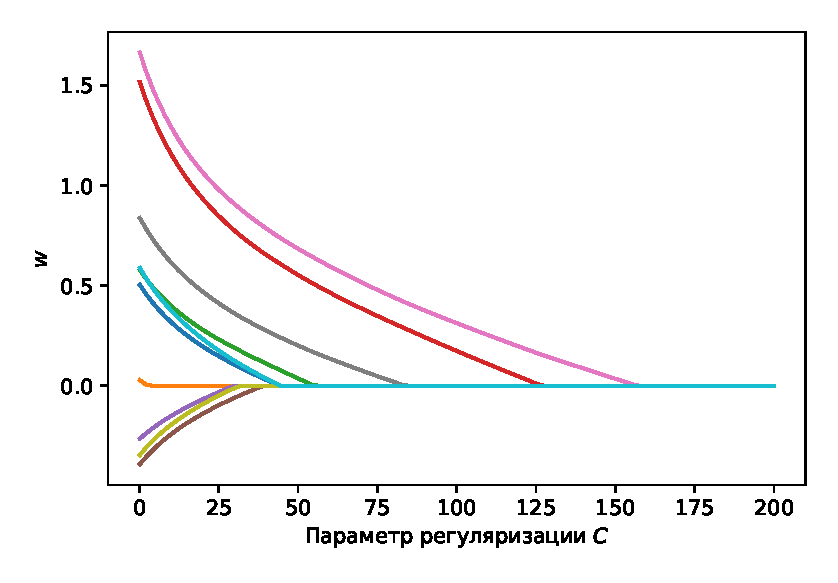
\includegraphics[width=0.5\textwidth]{../figures/log_reg_cs_exp.eps}
	\caption{Sample figure caption.}
	\label{fig:fig1}
\end{figure}

\subsection{Tables}
See awesome Table~\ref{tab:table}.

The documentation for \verb+booktabs+ (`Publication quality tables in LaTeX') is available from:
\begin{center}
	\url{https://www.ctan.org/pkg/booktabs}
\end{center}


\begin{table}
	\caption{Sample table title}
	\centering
	\begin{tabular}{lll}
		\toprule
		\multicolumn{2}{c}{Part}                   \\
		\cmidrule(r){1-2}
		Name     & Description     & Size ($\mu$m) \\
		\midrule
		Dendrite & Input terminal  & $\sim$100     \\
		Axon     & Output terminal & $\sim$10      \\
		Soma     & Cell body       & up to $10^6$  \\
		\bottomrule
	\end{tabular}
	\label{tab:table}
\end{table}

\subsection{Lists}
\begin{itemize}
	\item Lorem ipsum dolor sit amet
	\item consectetur adipiscing elit.
	\item Aliquam dignissim blandit est, in dictum tortor gravida eget. In ac rutrum magna.
\end{itemize}


\bibliographystyle{unsrtnat}
\bibliography{references}

\end{document}